\documentclass{amsart} 
\usepackage{amsmath}
\usepackage{verse}
\DeclareMathOperator*{\argmax}{arg\,max}
\DeclareMathOperator*{\argmin}{arg\,min}
\usepackage{graphicx}
\graphicspath{{./}}
\usepackage[fontsize=14pt]{scrextend}
\usepackage{hyperref}
\usepackage{csvsimple}
\usepackage{epigraph}
\title{People Everywhere Have Same Distribution on Media Influence}
\author{Zulfikar Moinuddin Ahmed}
\date{\today}
\begin{document}
\maketitle
\section{Meaning of Stability}

We are interested in examining Human Nature.  The Human Race is a Single Race with non-Africans on Earth sharing the same ancestors 75,000 years ago in a meta-tribe of East Africa.  Based on this strong fact of our sameness, the present author expects a much richer similarity of people than is expected by conventional theories of Social Sciences.  We support our viewpoint here by showing that the attitude towards media across the world has a strong regularity.

We stress emphasis that our result is a breakthrough result in the sense that it is both surprising and quantitatively strongly validated.  No one anywhere had ever suspected this sort of convergence across cultures, ethnicities and religions, and nations.

\section{Result}

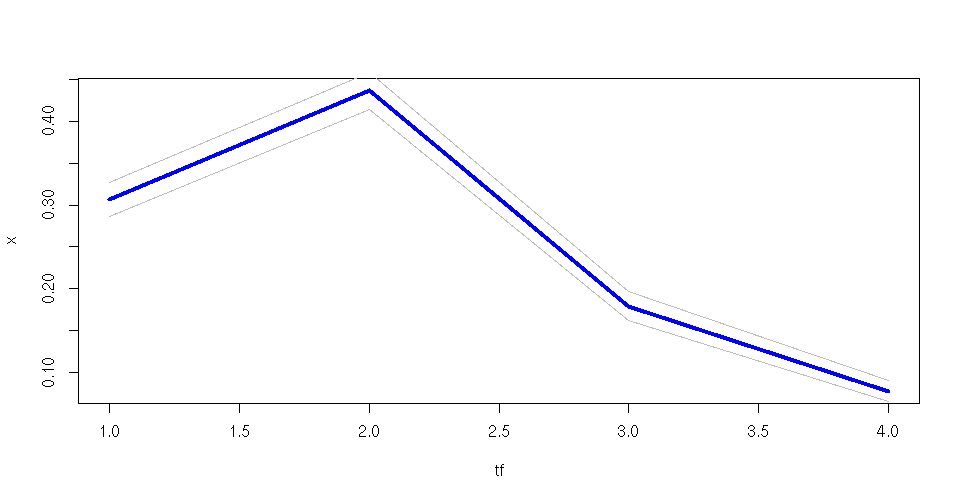
\includegraphics[scale=0.5]{medop.png}

The data are here:
% latex table generated in R 4.0.3 by xtable 1.8-4 package
% Wed Apr 14 05:21:47 2021
\begin{table}[ht]
\centering
\begin{tabular}{rrrr}
  \hline
 & x & sx & tf \\ 
  \hline
1 & 0.31 & 0.02 &   1 \\ 
  2 & 0.44 & 0.02 &   2 \\ 
  3 & 0.18 & 0.02 &   3 \\ 
  4 & 0.08 & 0.01 &   4 \\ 
   \hline
\end{tabular}
\end{table}

The density above is the percentage of population that believe media has (very good, good, bad, very bad) influence on society.  The data are from Pew 2014 survey.  The percentages are prominent.  Our discovery is that the standard deviation error from the mean curve is extremely tight.  

\section{Interpretation}
A random population chosen completely randomly without regard to country, ethnicity, religion, language will have the {\em same proportion} of the four different attitudes toward media.  This shows without much doubt that attitudes toward media opinion are independent of culture, language, ethnicity, nation, and other divisions, i.e. it depends only on Human Nature.


\section{Sampling with at least 20 countries}

As a further check to see how tight the distribution is, we sampled with rejection of those representing less than 20 countries.  The result was sharper.

\begin{verbatim}
> fmed.dens<-freq_dist_minspread(fmed.dat, ssize = 2000,
 nsampling=2000, minspread=20)
> fmed.curve<-stat_curve( fmed.dens)
> fmed.curve
          x          sx tf
1 0.3070380 0.010319988  1
2 0.4367128 0.010911329  2
3 0.1785194 0.008362823  3
4 0.0777298 0.006020627  4
\end{verbatim}


\end{document}